\documentclass[border=4pt]{standalone}
\usepackage{fontspec}
\usepackage{amsmath}
\usepackage{unicode-math}
\setmainfont{Latin Modern Roman}
\setmathfont{Latin Modern Math}
\usepackage{pgfplots}
\usepackage{pgfplotstable}
\pgfplotsset{compat=1.18}
\usepackage{tkz-euclide}
\usetikzlibrary{arrows.meta,calc,angles,quotes,patterns,3d,backgrounds}
\definecolor{ink}{HTML}{123428}
\definecolor{asy}{HTML}{475569}
\definecolor{mint}{HTML}{86e0bd}
\tikzset{asym/.style={asy, line width=0.9pt, dash pattern=on 5pt off 3.5pt},
         guide/.style={gray!70, line width=0.6pt, densely dotted},
         dot/.style={circle, inner sep=0pt, minimum size=5pt, draw=white, line width=0.5pt},
         odot/.style={circle, inner sep=0pt, minimum size=5.5pt, fill=white, line width=1pt},
         lab/.style={font=\footnotesize, inner sep=1.5pt, text=ink}}
\begin{document}
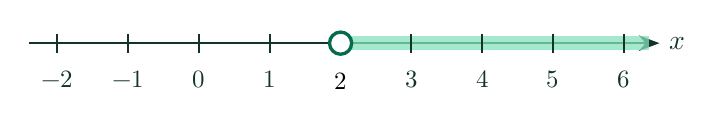
\begin{tikzpicture}[x=0.9cm, y=1cm]
\draw[ink, line width=0.8pt, -{Stealth[length=2.6mm]}] (-2.4,0) -- (6.5,0) node[right] {$x$};
\draw[mint, line width=5pt, opacity=0.75] (2.0,0) -- (6.35,0);
\draw[ink, line width=0.7pt] (-2,0.12) -- (-2,-0.12) node[below=3pt, font=\small] {$-2$};
\draw[ink, line width=0.7pt] (-1,0.12) -- (-1,-0.12) node[below=3pt, font=\small] {$-1$};
\draw[ink, line width=0.7pt] (0,0.12) -- (0,-0.12) node[below=3pt, font=\small] {$0$};
\draw[ink, line width=0.7pt] (1,0.12) -- (1,-0.12) node[below=3pt, font=\small] {$1$};
\draw[ink, line width=0.7pt] (3,0.12) -- (3,-0.12) node[below=3pt, font=\small] {$3$};
\draw[ink, line width=0.7pt] (4,0.12) -- (4,-0.12) node[below=3pt, font=\small] {$4$};
\draw[ink, line width=0.7pt] (5,0.12) -- (5,-0.12) node[below=3pt, font=\small] {$5$};
\draw[ink, line width=0.7pt] (6,0.12) -- (6,-0.12) node[below=3pt, font=\small] {$6$};
\node[circle, inner sep=0pt, minimum size=8pt, draw={rgb,255:red,4;green,107;blue,77}, line width=1.2pt, fill=white] at (2.0,0) {};
\node[font=\small, fill=white, inner sep=1pt] at (2.0,-0.48) {$2$};
\end{tikzpicture}
\end{document}
